\documentclass[
    preprint,
    12pt,
    letterpaper,
    longbibliography,
    nofootinbib,
    amsmath,
    amssymb,
    amsfonts,
]{revtex4-1}
\usepackage[utf8x]{inputenc}
\usepackage[T1]{fontenc}
\usepackage{lmodern}
\usepackage{enumerate}
\usepackage{graphicx}
\usepackage{hyperref}
\usepackage{epigraph}
\usepackage{mathpazo}
\usepackage{bm}

\newcommand{\m}[1]{\begin{bmatrix}#1\end{bmatrix}}
\newcommand{\vecof}[1]{\begin{pmatrix}#1\end{pmatrix}}
\newcommand{\tx}[1]{\text{#1}}
\newcommand{\pn}[1]{\left(#1\right)}
\newcommand{\abs}[1]{\left|#1\right|}
\newcommand{\norm}[1]{\left|\left|#1\right|\right|}
\newcommand{\bk}[1]{\left[#1\right]}
\newcommand{\abk}[1]{\left\langle#1\right\rangle}
\newcommand{\floor}[1]{\left\lfloor#1\right\rfloor}
\newcommand{\ceil}[1]{\left\lceil#1\right\rceil}
\newcommand{\set}[1]{\left\{#1\right\}}
\newcommand{\ellipsis}{\,\ldots}
\newcommand{\given}{\,|\,}
\newcommand{\where}{\mid}
\newcommand{\bbm}[1]{\mathbb{#1}}
\newcommand{\impl}{\rightarrow}
\newcommand{\dubimpl}{\leftrightarrow}
\newcommand{\calm}[1]{\mathcal{#1}}
\newcommand{\obar}[1]{\overline{#1}}
\newcommand{\lcm}{\text{lcm}}

\let\origfootnote\footnote
\renewcommand{\footnote}[1]{%
   \begingroup%
   \renewcommand{\footnotesize}{\fontsize{10pt}{8pt}\selectfont}%
   \origfootnote{#1}%
   \endgroup%
}

\begin{document}

\title{An Exploration of Bayesian Neural Networks}
\author{Evan Hubinger}
\affiliation{Harvey Mudd College}
\date{\today}

\maketitle

% Perhaps you will find yourself interested in a data set or a paper that requires
% Bayesian techniques slightly beyond the scope of our course. You will spend
% more time devoted to the description of the actual mathematics, with perhaps
% an implementation with parts or all of the new methodology either on this data
% set or a simulated data set.

% I’m thinking around 5-10 pages.

% noise_sd ~= 0.042722514277730474

\section{Introduction}

The idea of a Bayesian neural network dates back to Neal (1995)\cite{neal}, but has only relatively recently come to prominence with the rise of the use of deep neural networks by organizations such as DeepMind, Google Brain, and OpenAI. Bayesian neural networks are based on the idea of turning a standard neural network into a hierarchical Bayesian model. Thus, we will begin our exploration of Bayesian neural networks by delving into the workings of a traditional neural network.

\section{Traditional Neural Networks}

Conceptually, a neural network is simply a particular type of universal function approximator, which takes in some data $\bm x$ and outputs some $\bm y$. There are many different types of neural networks, but for the purposes of this paper we will focus on standard feed-forward networks, which operate as follows.

Suppose we are given some input data $\bm x$. Let $\bm a_0 = \bm x$. Then, where $W_0$ is some weight matrix and $\bm b_0$ is some bias vector, compute
\[
    \bm z_1 = \bm x^T W_0 + \bm b_0
\]
and, where $f$ is some nonlinear function (called an activation function), compute
\[
    \bm a_1 = f(\bm z_1)
\]
where $f$ is (usually) applied element-wise. We call the dimensionality of $\bm z_1$ the number of ``neurons'' in the layer. Then, we repeat the above process on $\bm a_1$ using new weights $W_1$ and biases $\bm b_0$. Finally, let $\bm y = \bm a_n$ where $n$ is the number of layers in the neural network.

This produces a model which maps input data $\bm x$ to output $\bm y$. Tuning the parameters of this sort of model is typically done via some variant of stochastic gradient descent.

\section{Bayesian Neural Networks}

We can turn the above traditional neural network into a Bayesian neural network by putting priors on the weights and biases in the model. For example, let
\begin{align*}
    & W_i \sim N(0, \bbm 1) \\
    & \bm b_i \sim N(\bm 0, \bm 1)
\end{align*}
Additionally, to allow for noise in the model, let
\[
    \bm y \sim N\pn{\bm a_n, \sigma (\bm 1)}
\]
where $\sigma$ is a scalar representing the amount of noise in the model.

This produces a hierarchical Bayesian model. Updating this model with training data produces a posterior distribution over $\bm y$ which can be used to model the relationship between $\bm x$ and $\bm y$.

Since Bayesian neural networks are full, hierarchical Bayesian models, they can be used to produce more than simply point estimates. In particular, the posterior model can be sampled from to produce estimates of the model's uncertainty.

\section{Our Experiment}

\subsection{Setup}

To showcase Bayesian neural networks, we will explore a toy Bayesian neural network. We will be using Edward for this, a Python library for probabilistic programming built on TensorFlow.\cite{edward} The example we will be using is modified from Edward's tutorials.\cite{tutorial} The full code for everything we will be doing can be accessed online on GitHub.\cite{code}

We will be attempting to model the true data distribution
\[
    y \sim N\pn{\sin(\pi(x+1)), 0.05}
\]
For our training data, we sampled 100 data points uniformly on the range $x \in [-1, -0.1]$ and 100 data points uniformly on the range $x \in [0.1, 1]$. This allows us to leave the range $x \in [-0.1, 0.1]$ empty to test our model's ability at interpolation. See Figure \ref{fig:1} for the sampled training data.

\begin{figure}
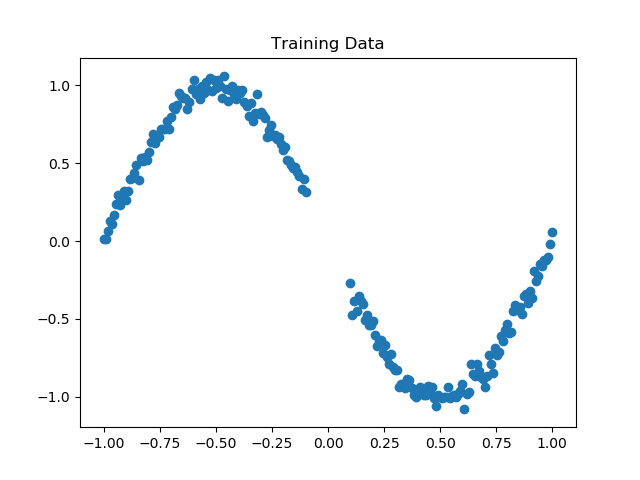
\includegraphics{Figure_1.png}
\caption{Training data sampled using the methodology given above.}
\label{fig:1}
\end{figure}

\subsection{Procedure}

We then constructed a three-layer feed-forward Bayesian neural network with 10 neurons per layer and activation function $f(x) = \tanh(x)$. We used standard normal priors for the weights and biases and modeled $y \sim N(\bm a_n, \sigma)$. We estimated $\sigma$ from the data using a finite difference method, which gave the approximation $\sigma \approx 0.0427$, which is very close to the true value $\sigma = 0.05$. To visualize our prior model, we sampled 10 different sets of weights and biases from the prior distribution and plotted the resulting models in Figure \ref{fig:2}.

\begin{figure}
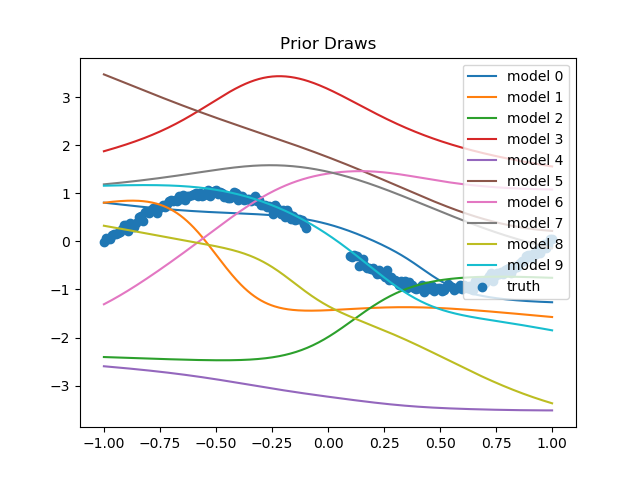
\includegraphics{Figure_2.png}
\caption{10 draws from the prior model distribution plotted alongside the actual data.}
\label{fig:2}
\end{figure}

\newpage

While the large variety of different prior model curves shown in Figure \ref{fig:2} demonstrate that our prior is clearly very uncertain, they also demonstrate the power of our Bayesian neural network in terms of the large number of different types of relationships it is able to model. In particular, we see fairly linear models (model 5), models with something close to a step function in them (model 1), and even approximately normal models (model 3).

We then updated our network using the training data given above. Since an analytical approach to computing the posterior is impossible, we approximated the posterior using variational inference. Specifically, we used variational expectation maximization with a Kullback-Leibler divergence loss function to approximate model parameters.\cite{klpq} We ran 1500 iterations of variational inference with 15 samples per iteration.

\newpage

\subsection{Results}

To visualize our posterior, we again sampled 10 different sets of weights and biases, the resulting models of which are plotted in Figure \ref{fig:3}. Based on the posterior draws in Figure \ref{fig:3}, we can see that our model has captured the basic shape of the underlying distribution over the range with data, and has even managed to produce a fairly good interpolation for the $[-0.1, 0.1]$ range where no data was given.

\begin{figure}
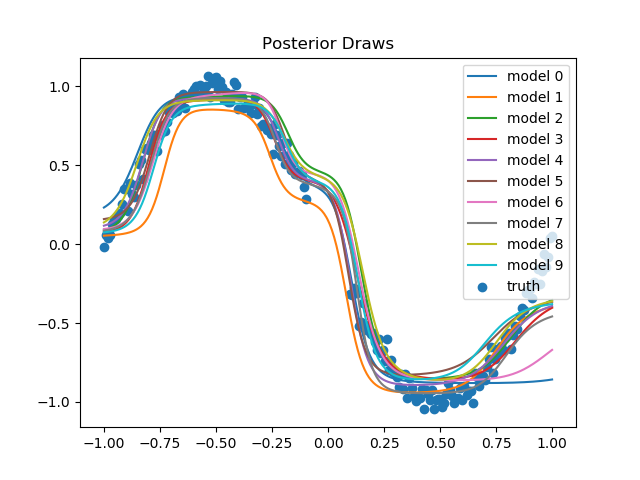
\includegraphics{Figure_3.png}
\caption{10 draws from the posterior model distribution plotted alongside the actual data.}
\label{fig:3}
\end{figure}

\newpage

If we take the posterior mean to be our point estimate $\hat y = \bar y$, we can compare our model's mean estimate to the actual $X, y$ data. See Figure \ref{fig:4} for the posterior means plotted alongside the ground truth.

One interesting thing to note about our posterior is that it seems to have produced a better, more confident fit for the negative $x$ values than the positive $x$ values. This is due to the fact that the expectation maximization strategy we are using to tune our parameters is good at reaching local minima but necessarily global minima. Thus, if run many times, it tends to produce a very good approximation for either the negative values or the positive values, but not both, since each one is modeled well by a different local minima.

\begin{figure}
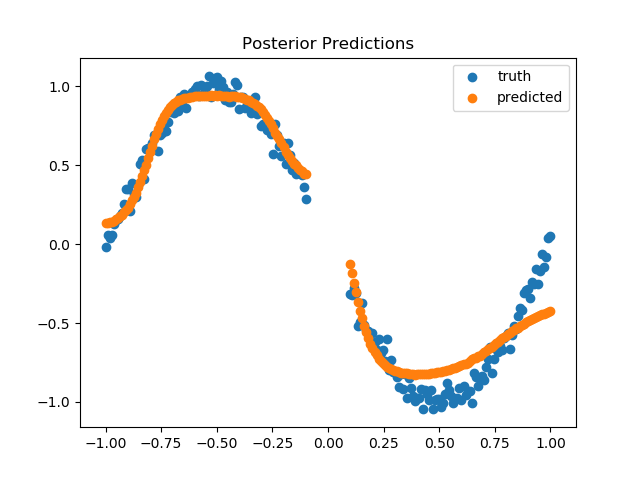
\includegraphics{Figure_4.png}
\caption{Posterior mean estimates plotted alongside the actual data.}
\label{fig:4}
\end{figure}

\newpage

Since we have a full posterior distribution, we can also compare samples from the posterior to the actual data using various different metrics. This type of posterior analysis is known as a posterior predictive check.\cite{ppc} One example metric is simply $\bar y$, which we can calculate should be approximately
\begin{align*}
    & \bbm E\bk{\bar y \where x \in [-1, 1]} \\
    & = \bbm E\bk{\sin(\pi(x+1)) \where x \in [-1, 1]} \\
    & = 0
\end{align*}

A plot of the posterior $\bar y$ distribution estimated based on 400 samples alongside the actual data $\bar y$ is given in Figure \ref{fig:5}. From Figure \ref{fig:5}, we can see that the actual $\bar y$ is relatively close to the center of the posterior $\bar y$ distribution, and is assigned a relatively high posterior probability. Thus, we can be fairly confident that, at least with respect to $\bar y$, our posterior is properly assigning a large probability to the true distribution.

\begin{figure}
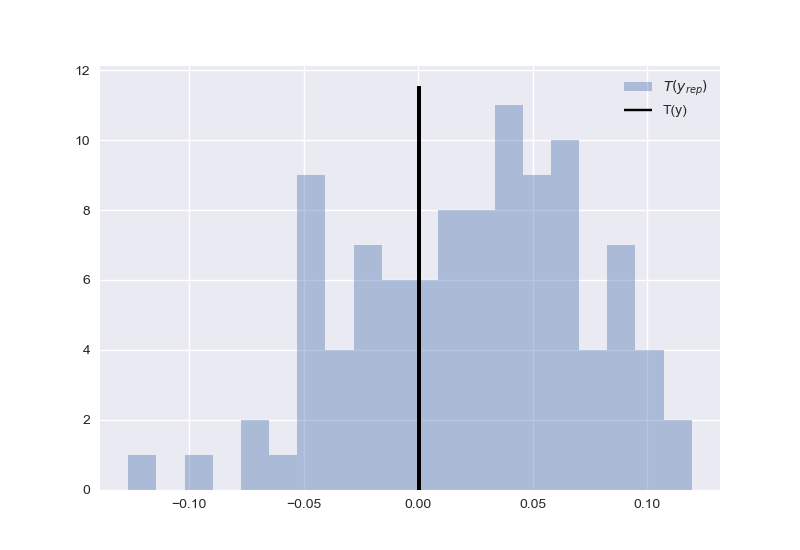
\includegraphics[scale=0.8]{Figure_5.png}
\caption{Actual $\bar y$ plotted alongside an estimate of the posterior $\bar y$ distribution.}
\label{fig:5}
\end{figure}

\section{Conclusion}

As demonstrated by our experiment, Bayesian neural networks are a powerful tool for modeling unknown relationships. Specifically, we demonstrated that for the particular problem where $y$ is a sinusoidal function of $x$ plus random noise, a simple three-layer Bayesian neural network with 10 neurons per layer is able to correctly approximate the true relationship.

Furthermore, in comparison to traditional neural networks, we have shown how Bayesian neural networks can be significantly more informative, by allowing for prior and posterior draws as well as posterior predictive checks. For this reason, we believe that Bayesian neural networks are currently underutilized in machine learning applications where the informativeness of the model---such as knowing the model's uncertainty---is critical.

\bibliography{bnns_sources}

\end{document}
